\documentclass[hyperref={pdfpagelayout=SinglePage}]{beamer}
\usetheme{Warsaw}
\usecolortheme{default}
\usefonttheme[onlymath]{serif}
\usepackage[utf8]{inputenc}
\usepackage[spanish,activeacute]{babel}

\usepackage{graphicx}
\usepackage{fancyhdr}
\usepackage{float}
\usepackage{adjustbox}
\usepackage{subfigure}
\usepackage{amsmath}
\usepackage{ragged2e}

\usepackage{color}
\usepackage{listings}
\lstset{ %
basicstyle=\footnotesize,       % the size of the fonts that are used for the code
numbers=none,                   % where to put the line-numbers
numberstyle=\footnotesize,      % the size of the fonts that are used for the line-numbers
stepnumber=1,                   % the step between two line-numbers. If it is 1 each line will be numbered
numbersep=10pt,                  % how far the line-numbers are from the code
backgroundcolor=\color{white},  % choose the background color. You must add \usepackage{color}
showspaces=false,               % show spaces adding particular underscores
showstringspaces=false,         % underline spaces within strings
showtabs=false,                 % show tabs within strings adding particular underscores
frame=single,           % adds a frame around the code
tabsize=4,          % sets default tabsize to 2 spaces
captionpos=b,           % sets the caption-position to bottom
breaklines=true,        % sets automatic line breaking
breakatwhitespace=false,    % sets if automatic breaks should only happen at whitespace
escapeinside={\%*}{*)}          % if you want to add a comment within your code
}
\renewcommand{\lstlistingname}{Código}
\renewcommand\spanishtablename{Tabla}

\expandafter\def\expandafter\insertshorttitle\expandafter{%
  \insertshorttitle\hfill%
  \insertframenumber\,/\,\inserttotalframenumber}

\title{Autómatas Celulares}
\subtitle{Trabajo Practico Nro. 2}
%\author{Grupo 3}
\author{Badi Leonel, Buchhalter Nicolás Demián y Meola Franco Román}
\subject{Simulación de Sistemas}
\date{\today}

\makeatletter
\@addtoreset{subfigure}{framenumber}
\makeatother

\begin{document}

\renewcommand{\figurename}{Grafico}

\begin{frame}[plain]
    \frametitle{} 
    \titlepage
\end{frame}

\section{Fundamentos}

\subsection{Introducción}

\begin{frame}
\frametitle{Fundamentos}
\framesubtitle{Introducción}
\begin{itemize}
	\item Autómata Off-Latice de Bandadas de Agentes Autopropulsados.
	\item Basado en el algoritmo del trabajo de \textit{Novel type of phase transition in a system of self-driven particles}.
	\item Cada agente será representado por un vector de velocidad cuyo origen estará ubicado en la posición de la partícula para cada tiempo de la simulación $t$.
\end{itemize}
\end{frame}

\subsection{Variables relevantes}

\begin{frame}
\frametitle{Fundamentos}
\framesubtitle{Variables relevantes}
\begin{itemize}
	\item $N$ : cantidad de agentes
	\item $L$ : longitud del lado del área de simulación
	\item $r_{c}$ : radio de interacción de las partículas
	\item $v$ : módulo de la velocidad
	\item $\rho = \frac{N}{L^2}$ : densidad
	\item $\eta$ : amplitud del ruido
	\item $v_{a}$ : parámetro de orden
	\item Nos interesa obtener las curvas de  $v_{a}$ en función de $\eta$ y $\rho$.
\end{itemize}
\end{frame}

\section{Implementación}

\subsection{Generación de los agentes}

\begin{frame}
\frametitle{Implementación}
\framesubtitle{Generación de los agentes}
\begin{itemize}
	\item Posiciones $(x,y)$ aleatorias para cada agente.
	\item $r = 0.1$
	\item $v_{cte} = 0.3$
	\item $\theta_{0} = rand() * 2\pi$ (ángulo inicial aleatorio)
	\item $\delta_{\theta} = {(rand() * \eta) - \frac{\eta}{2}} $
\end{itemize}
\end{frame}

\subsection{Modelo del Agente}

\begin{frame}
\frametitle{Implementación}
\framesubtitle{Modelo del Agente}
Una partícula está compuesta por:
\begin{itemize}
	\item $(x,y)$: Posición 
	\item $|v|$: Módulo de la velocidad
	\item $\theta$ : Ángulo
	\item Lista de agentes vecinos
\end{itemize}
\end{frame}

\subsection{Modelo del Sistema}

\begin{frame}
\frametitle{Implementación}
\framesubtitle{Modelo del Sistema}
El sistema está compuesto por:
\begin{itemize}
	\item $N$ 
	\item $L$
	\item $r_{c}$
	\item Longitud del lado de un elemento de la grilla
	\item Lista de partículas
	\item Arreglo de listas de partículas
\end{itemize}
\end{frame}

\subsection{Simulación}

\begin{frame}[fragile]
\frametitle{Implementación}
\framesubtitle{Simulación}
\begin{lstlisting}[language=Java, caption = Algoritmo de simulación de partículas.]
for(Frame frame : frames) {
	List<Particle> particles = calculateNeighbours();
	for(Particle particle : particles) {
		particle.updateAngleAndPosition();
		if(particle.isInBorderPosition()) {
			particle.makePeriodicTraslation();
		}
	}
	saveFrameData();
}
\end{lstlisting}
\end{frame}

\begin{frame}
\frametitle{Implementación}
\framesubtitle{Visualización}
\begin{itemize}
	\item La simulación y la visualización son independientes
	\item El algoritmo de simulación escribe un archivo \texttt{.tsv} con los siguientes datos:
\begin{itemize}
\item $(x,y)$
\item $r$
\item Color RGB para indicar las velocidades, donde R es la componente en el eje Y y G es la componente en eje X
\end{itemize}
\item Por último, se carga en \texttt{Ovito} el archivo de salida\texttt{.tsv} para hacer la visualización
\end{itemize}
\end{frame}

\section{Resultados}

\subsection{Tablas}

\begin{frame}
\frametitle{Resultados}
\framesubtitle{$N = 40$, $L = 3.1$ y $r_{c} = 1$}
\begin{center}
\begin{table}[h]
\centering
\adjustbox{max height=\dimexpr\textheight-3.0cm\relax,
           max width=\textwidth}{
\begin{tabular}{cc}
\hline
\textbf{$\eta$} & \textbf{$v_{a}$}\\ \hline
0.0&1.00000\\
0.5&0.98799\\
1.0&0.95777\\
1.5&0.89056\\
2.0&0.82847\\
2.5&0.71321\\
3.0&0.55152\\
3.5&0.53482\\
4.0&0.42995\\
4.5&0.38458\\
5.0&0.11822\\
\end{tabular}
}
\caption{Datos de la curva de $v_{a}$ para $N = 40$, $L = 3.1$ y $r_{c} = 1$.}
\end{table}
\end{center}
\end{frame}

\begin{frame}
\frametitle{Resultados}
\framesubtitle{$N = 400$, $L = 10$ y $r_{c} = 1$}
\begin{center}
\begin{table}[h]
\centering
\adjustbox{max height=\dimexpr\textheight-3.0cm\relax,
           max width=\textwidth}{
\begin{tabular}{cc}
\hline
\textbf{$\eta$} & \textbf{$v_{a}$}\\ \hline
0.0&0.99999\\
0.5&0.97909\\
1.0&0.87444\\
1.5&0.78458\\
2.0&0.70671\\
2.5&0.25537\\
3.0&0.46229\\
3.5&0.35985\\
4.0&0.13354\\
4.5&0.06530\\
5.0&0.04682\\
\end{tabular}
}
\caption{Datos de la curva de $v_{a}$ para $N = 400$, $L = 10$ y $r_{c} = 1$.}
\end{table}
\end{center}
\end{frame}

\begin{frame}
\frametitle{Resultados}
\framesubtitle{$N = 10000$, $L = 50$ y $r_{c} = 1$}
\begin{center}
\begin{table}[h]
\centering
\adjustbox{max height=\dimexpr\textheight-3.0cm\relax,
           max width=\textwidth}{
\begin{tabular}{cc}
\hline
\textbf{$\eta$} & \textbf{$v_{a}$}\\ \hline
0.0&0.92861\\
0.5&0.07030\\
1.0&0.44647\\
1.5&0.46268\\
2.0&0.26689\\
2.5&0.20727\\
3.0&0.03786\\
3.5&0.05376\\
4.0&0.00901\\
4.5&0.00760\\
5.0&0.00412\\
\end{tabular}
}
\caption{Datos de la curva de $v_{a}$ para $N = 10000$, $L = 50$ y $r_{c} = 1$.}
\end{table}
\end{center}
\end{frame}

\subsection{Gráfico}

\begin{frame}
\frametitle{Resultados}
\framesubtitle{Gráfico}
\begin{figure}[H]
        \centering
        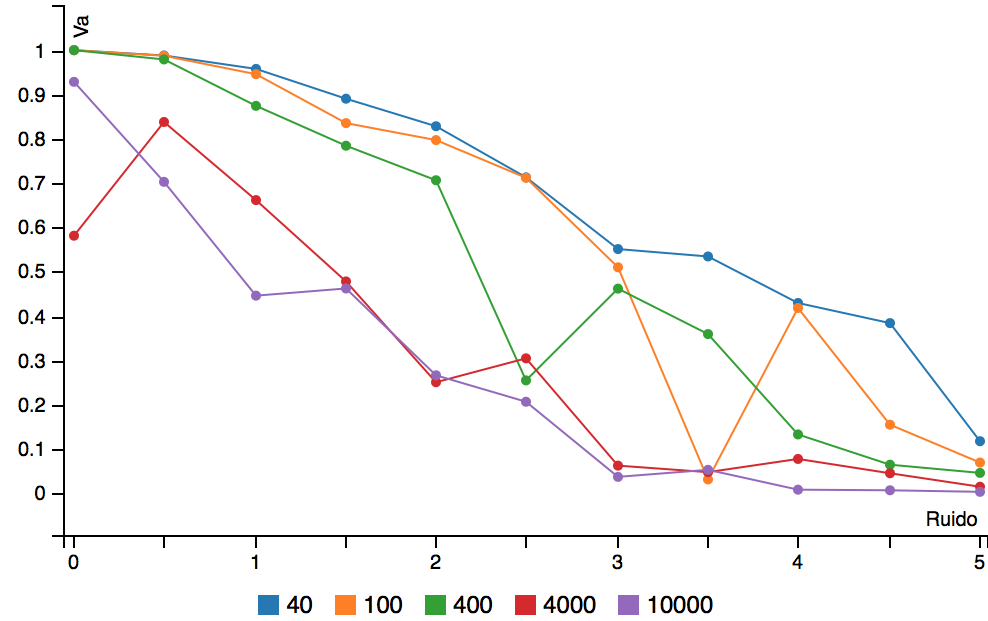
\includegraphics[width=\textheight]{graphic.png}
        \caption{Gráfico de la curva de $v_{a}$ para distintos valores de $N$, $L$ y $\eta$. http://bl.ocks.org/lbadi/05bfacbb96e14df499a7ef18b37ca2cc}
\end{figure}
\end{frame}

\subsection{Animaciones}

\begin{frame}
\frametitle{Resultados}
\framesubtitle{Animaciones}
\begin{figure}[H]
        \centering
        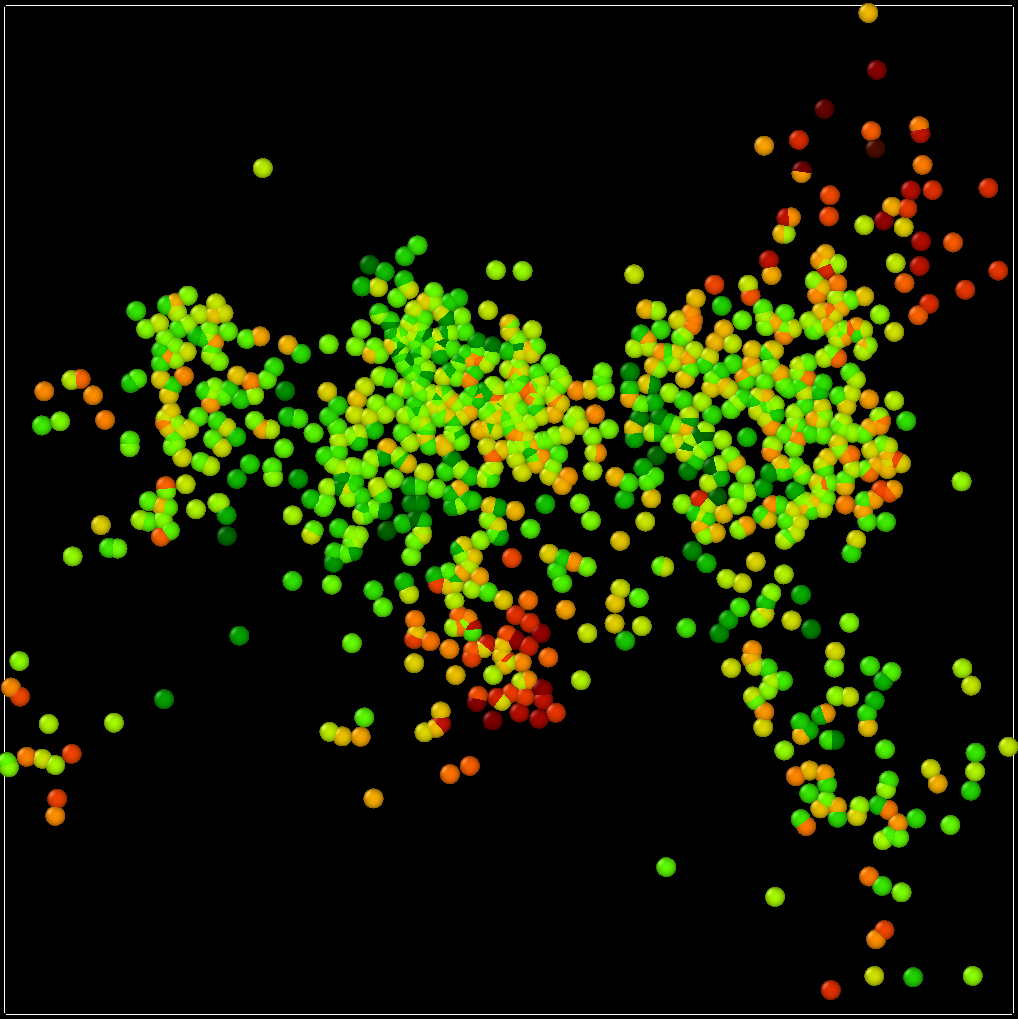
\includegraphics[width=0.70\textheight]{screenshot.png}
        \caption{Ver archivos \texttt{.avi} en la demostración en vivo.}
\end{figure}
\end{frame}

\end{document}